\documentclass[10pt,twocolumn,letterpaper]{article}

\usepackage{cvpr}
\usepackage{times}
\usepackage{epsfig}
\usepackage{graphicx, color, xcolor}
\usepackage{amsmath}
\usepackage{amssymb}
\usepackage{bm}
\usepackage[utf8]{inputenc}
\usepackage{fancyhdr}
\usepackage{graphicx}
\usepackage[brazil]{babel}
\usepackage{lipsum}
\usepackage{float}
\setlength{\headheight}{1.5cm}

\fancypagestyle{plain}
\lhead{
\includegraphics[width=5cm,height=2cm]{logoFT.png}}
\rhead{
\includegraphics[width=5cm,height=2cm]{logoUnB.png}}

\renewcommand{\headrulewidth}{1pt}%
}

% Changing the caption and 'References' names to Portuguese.
\addto\captionsenglish{
  \renewcommand{\figurename}{Figura}
  \renewcommand{\tablename}{Tabela}
  \renewcommand{\refname}{Referências bibliográficas}
}

% to-do: Using fontenc with T1 font encoding allows \hyphenation to take words with accents
% as arguments. However, fontenc with T1 mess up with words containing 'ã' in all \subsection{}
% commands.
% If someone knows how to fix it, tell me!
%
%\usepackage[T1]{fontenc}

% Put the words not correctly hyphenated down here. Words with accents must
% be manually hyphenated in the text itself using the '\-' separator. See the examples
% throughout this template.
\hyphenation{co-e-ren-te u-sa-do de-li-mi-ta-do-res a-cer-ca va-lo-res cor-res-pon-den-te re-fe-ren-ci-a-das co-lu-na co-lu-nas em-bo-ra u-ti-li-da-de pro-ce-di-men-to ex-pe-ri-men-to fi-gu-ras}

% If you comment hyperref and then uncomment it, you should delete
% egpaper.aux before re-running latex.  (Or just hit 'q' on the first latex
% run, let it finish, and you should be clear).
\usepackage[breaklinks=true,bookmarks=true]{hyperref}

\cvprfinalcopy % *** Uncomment this line for the final submission

%\def\cvprPaperID{****} % *** Enter the CVPR Paper ID here
%\def\httilde{\mbox{\tt\raisebox{-.5ex}{\symbol{126}}}}

% Pages are numbered in submission mode, and unnumbered in camera-ready
% \ifcvprfinal\pagestyle{empty}\fi
%\setcounter{page}{1}


\begin{document}
%%%%%%%%% TITLE
\title{Experimento 1: Simulações LTspice}

\author{Yuri Shumyatsky\\
% To save space, use either the email address or home page, not both
{\tt\small 231012826@aluno.unb.br}\\
% Matrícula do primeiro autor
{\tt\small 231012826}\\
% Turma
{\tt\small Turma T02}
\and
Aluno 2\\
{\tt\small aluno2@aluno.unb.br}\\
% Matrícula do segundo autor
{\tt\small 00/0000000}\\
% Turma
{\tt\small Turma A/D}
\and
Aluno 3\\
{\tt\small aluno3@aluno.unb.br}\\
% Matrícula do terceiro autor, se houver
{\tt\small 00/0000000}\\
% Turma
{\tt\small Turma A/D}
}

\maketitle
%\thispagestyle{empty}
\section{Procedimento experimental}

O experimento 1 consiste em uma familiarização com o software LTspice para simulações de circuitos. As primeiras simulações são de um circuito divisor de corrente, com $R_1 = 26k\Omega, R_2 = 28k\Omega, R_3 = 1k\Omega$

\begin{figure}[h]
\caption{Circuito divisor de corrente}
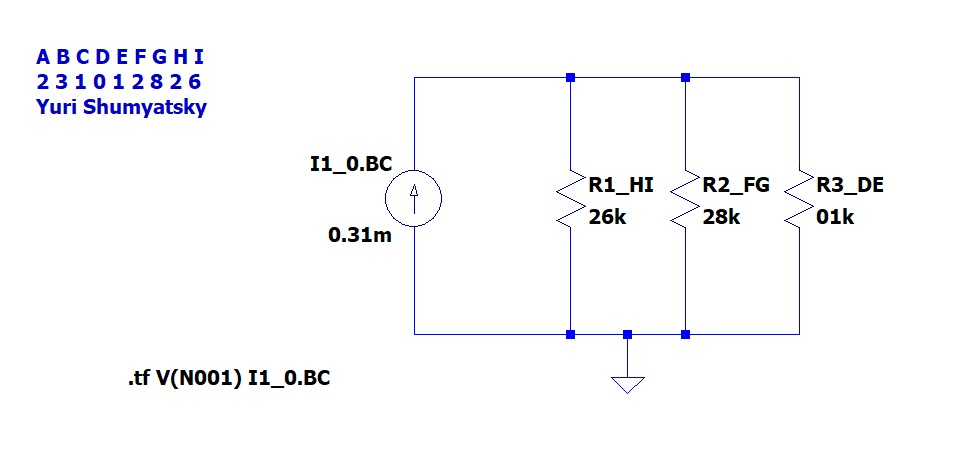
\includegraphics[scale=0.2]{figuras/fig1}
\end{figure}

Algumas simulações são feitas para um filtro RC passa altas com frequência de corte de 28kHz, no entanto. Essas são as Análises AC. Os valores dos componentes para esse circuito são $R_1=26k\Omega, C_1=0.219nF$ e uma fonte de tensão senoidal com amplitude de 1V.

\begin{figure}[h]
\caption{Circuito filtro passa-altas}
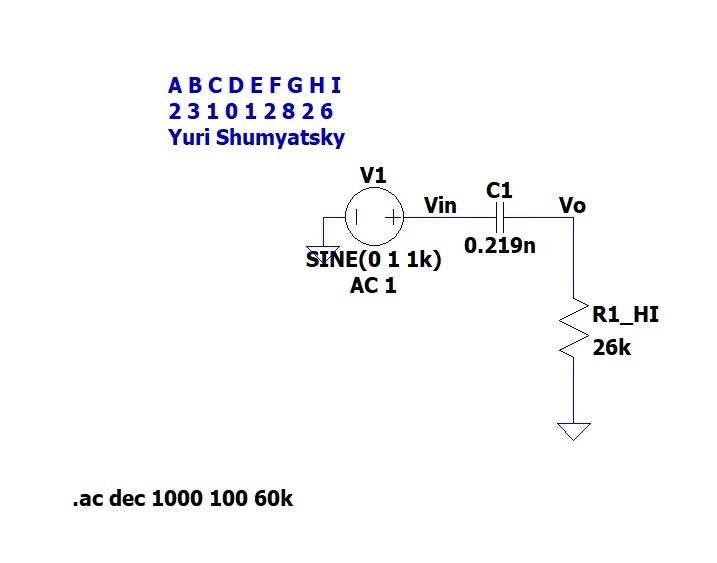
\includegraphics[scale=0.2]{figuras/fig2}
\end{figure}

%-------------------------------------------------------------------------
\section{Resultados e análises}

\subsection{ Análise de Ponto de Operação}

Para o divisor de corrente analisado, a resistência equivalente é de $0.93k\Omega$ e portanto as correntes $i_1, i_2, i_3$ podem ser calculadas usando a fórmula:

\[i_n = \frac{R_{eq}}{R_n}i\]

O que resulta em $i_1 = 0.01109mA$, $i_2 = 0.0103mA$, $i_3 = 0.288mA$. Além disso, o cálculo da tensão do nó N001 é simplesmente $U=R_{eq}i$, resultando em $U=0.2883V$

A análise de ponto de operação resultou em valores compatíveis com esses cálculos.

\begin{figure}[h]
\caption{Resultados análise DC op pnt}
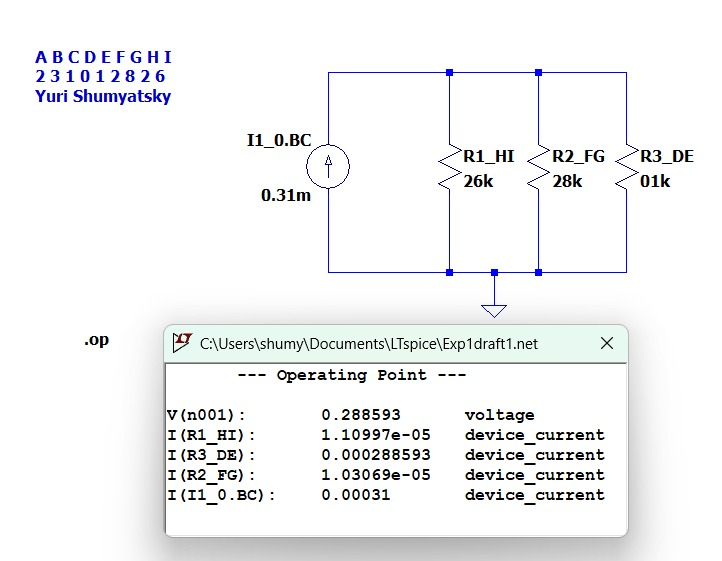
\includegraphics[scale=0.2]{figuras/fig3}
\end{figure}

\subsection{Análise Transiente}

Para a análise transiente, a fonte deixa de ser DC e passa a ser um sinal triangular com período de 2ms e amplitude de 0.31mA.

Seguem os gráficos das correntes.

\begin{figure}[h]
\caption{Correntes fonte e $R_1$}
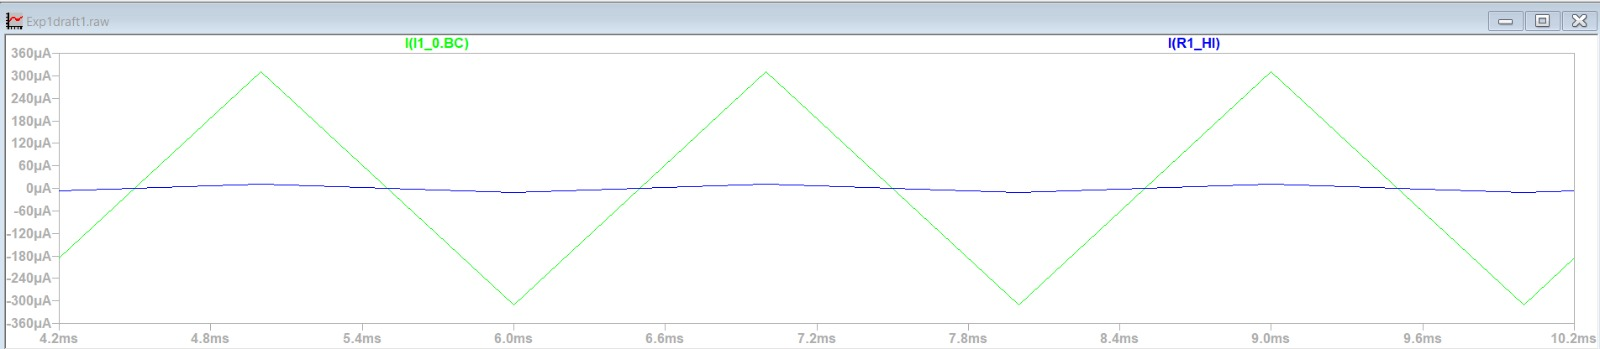
\includegraphics[scale=0.14]{figuras/fig4}
\end{figure}

\begin{figure}[h]
\caption{Correntes fonte e $R_2$}
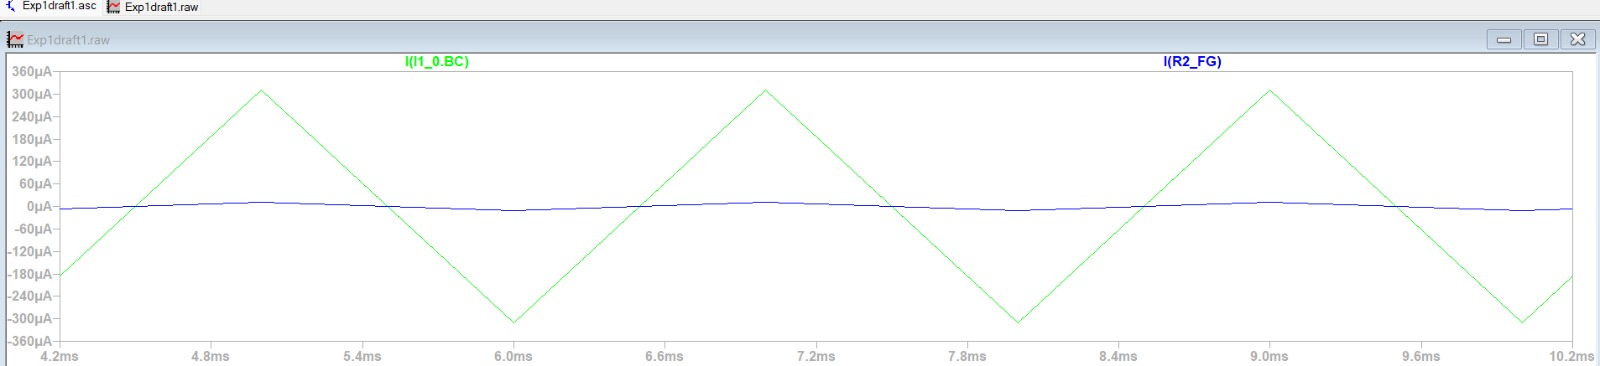
\includegraphics[scale=0.14]{figuras/fig5}
\end{figure}

\begin{figure}[h]
\caption{Correntes fonte e $R_3$}
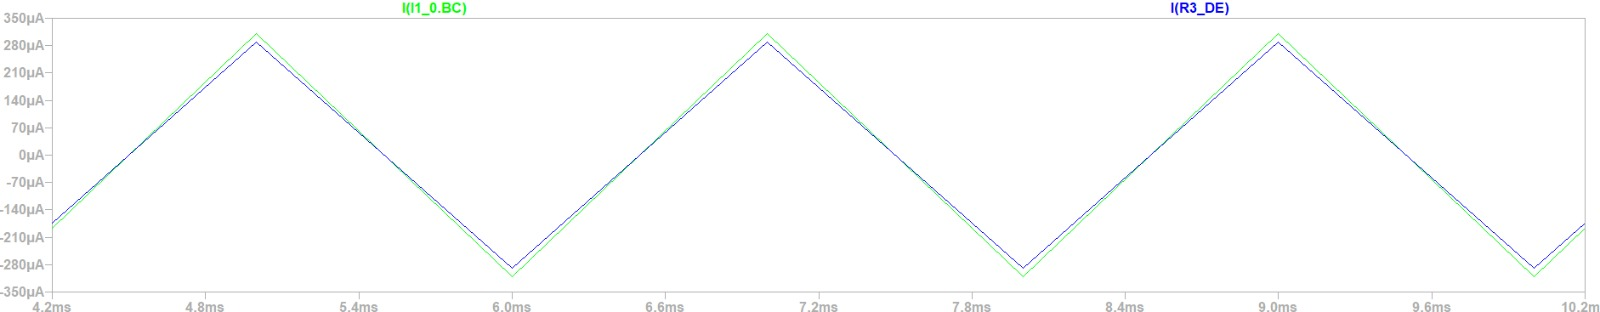
\includegraphics[scale=0.14]{figuras/fig6}
\end{figure}

O próximo gráfico mostra a validade da Lei das Correntes de Kirchhoff, ao comparar a corrente da fonte com a soma das correntes nos resistores.

\begin{figure}[h]
\caption{Validação da Lei das Correntes de Kirchhoff}
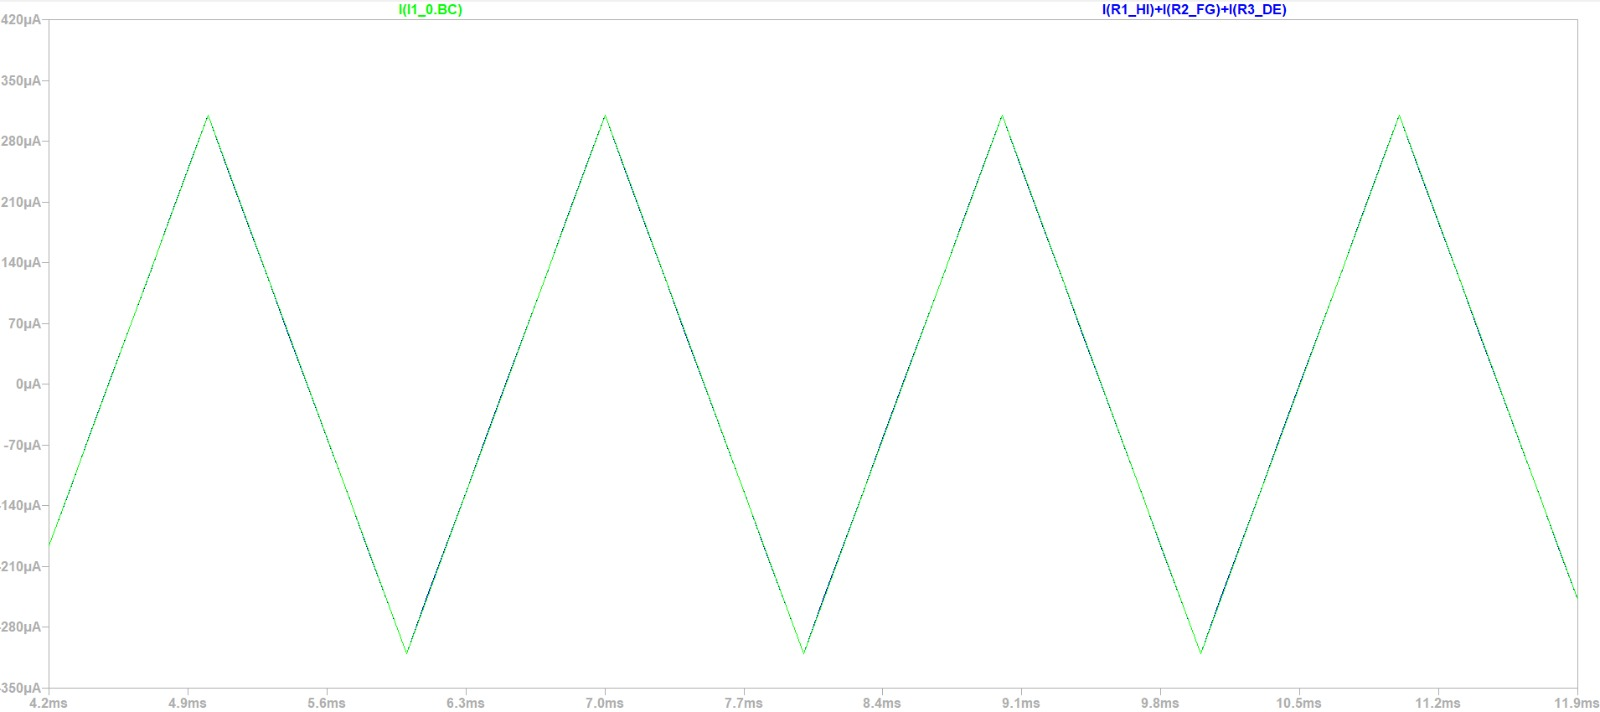
\includegraphics[scale=0.15]{figuras/fig7}
\end{figure}

De forma semelhante, a figura 8 mostra a validade do Teorema de Tellegen ao comparar as potências fornecidas e dissipadas na fonte e nas resistências.

\begin{figure}[h]
\caption{Validação do Teorema de Tellegen}
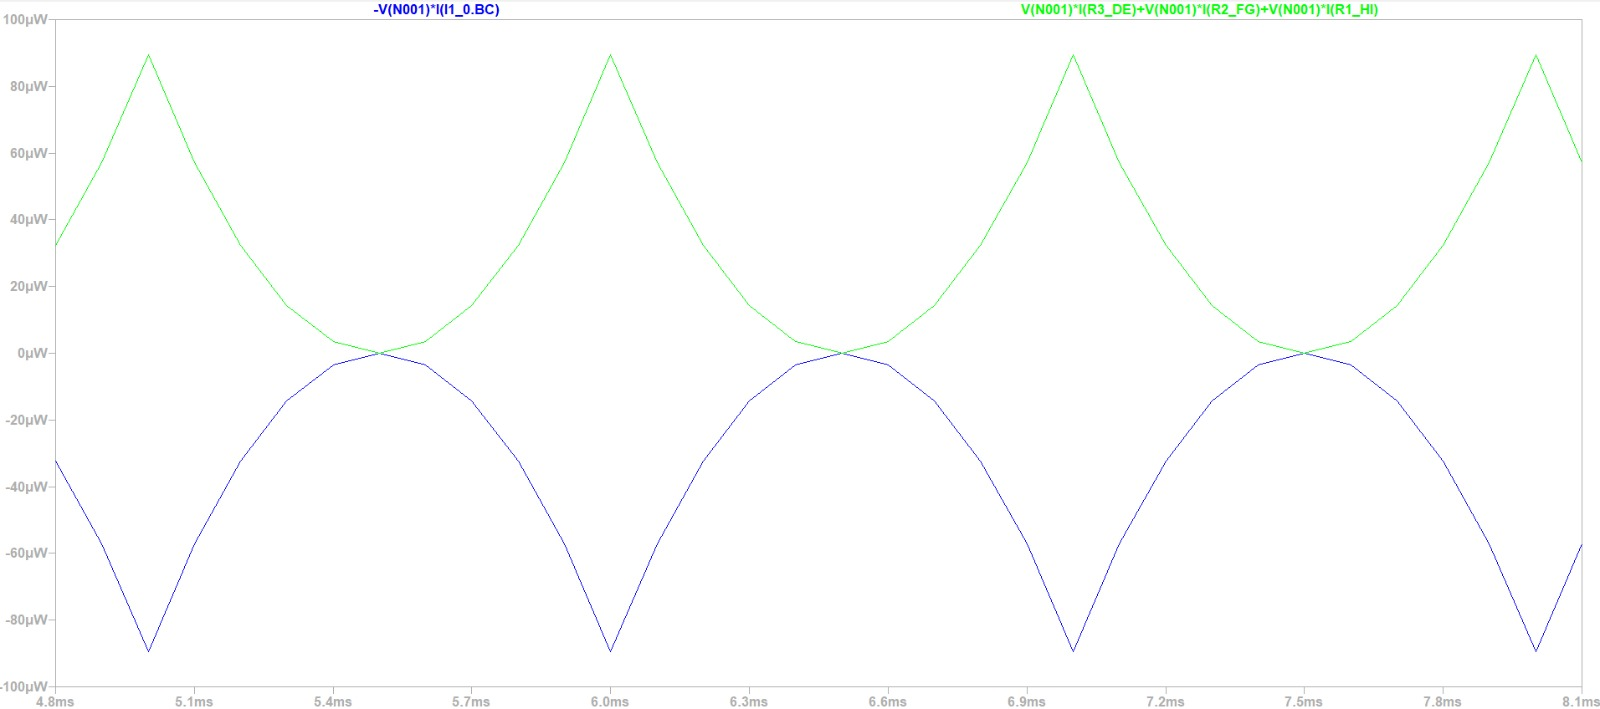
\includegraphics[scale=0.15]{figuras/fig8}
\end{figure}

\subsection{Análise AC}

Essa análise é feita sobre o circuito filtro passa-altas. Para calcular o valor da capacitância necessário para que a frequência de corte seja $28kHz$, usa-se a seguinte fórmula:

\[f_c=\frac{1}{2\pi RC} \implies C = \frac{1}{2\pi\cdot26\cdot28\cdot10^6}=0.219\cdot10^{-9}F\]

Assim, são plotadas as respostas em amplitude e em fase do circuito na Figura 9.

\begin{figure}[h]
\caption{Resultado Análise AC}
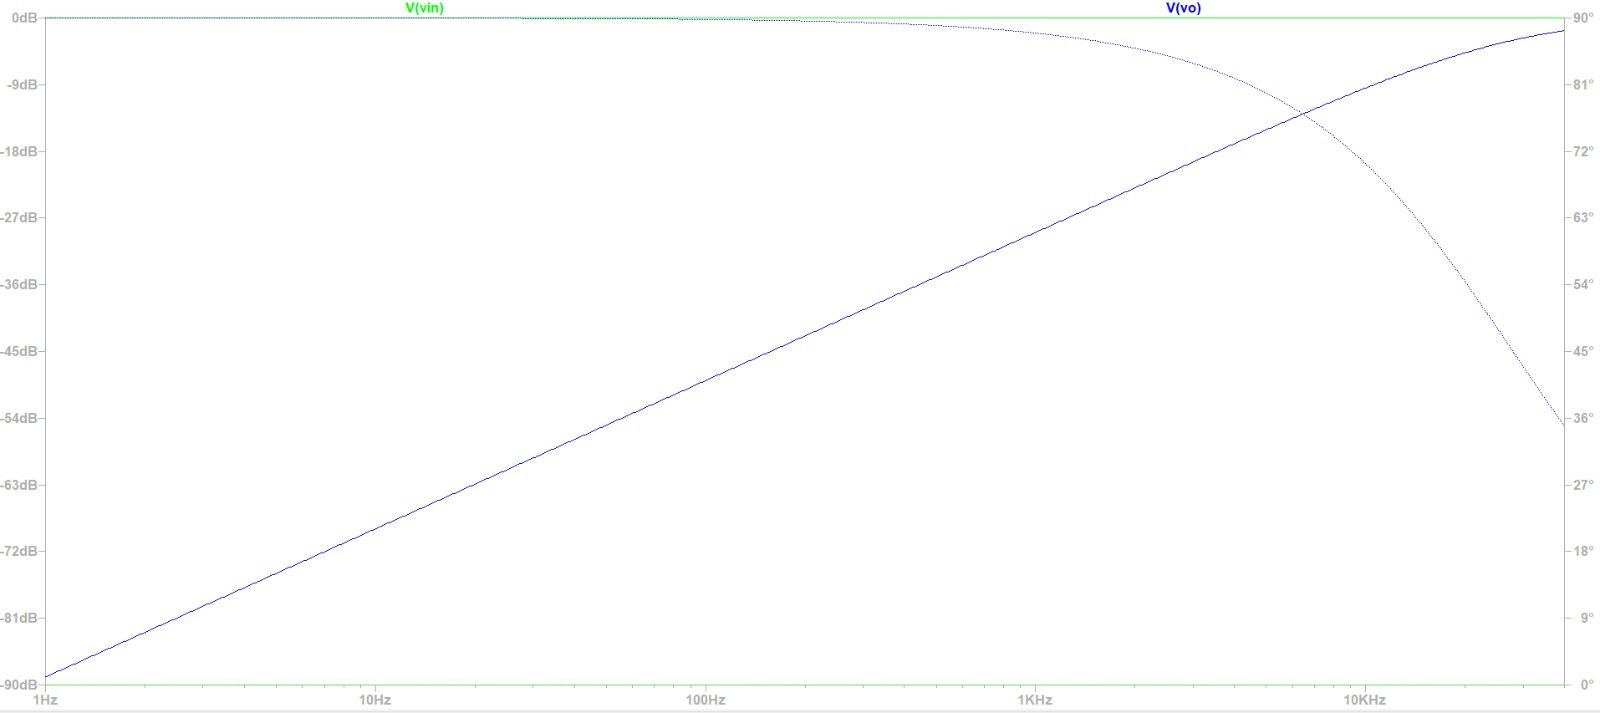
\includegraphics[scale=0.15]{figuras/fig9}
\end{figure}\newpage

Como $\frac{P_o}{P_i} = \frac{V_o}{V_i}\frac{I_o}{I_i} = |H(j\omega)|^2, H(j\omega) = \frac{j\omega RC}{1+j\omega RC}$, e na frequência de corte $\omega=\frac{1}{RC}$, $|H(jf_c)|^2 = 1/2$, o que na escala dB resulta em aproximadamente -3.01dB.

\begin{figure}[h]
\caption{Análise Fator Po/Pi}
\begin{center}
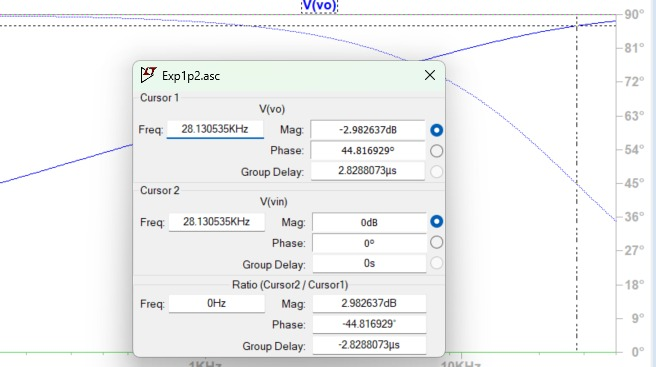
\includegraphics[scale=0.2]{figuras/fig13}
\end{center}
\end{figure}


Em seguida, é comparada a corrente fluindo pelo circuito com a curva calculada pelo LTspice através da fórmula:
\[I = C\cdot\frac{dV}{dt}\]

\begin{figure}[h]
\caption{Plotagem da corrente calculada}
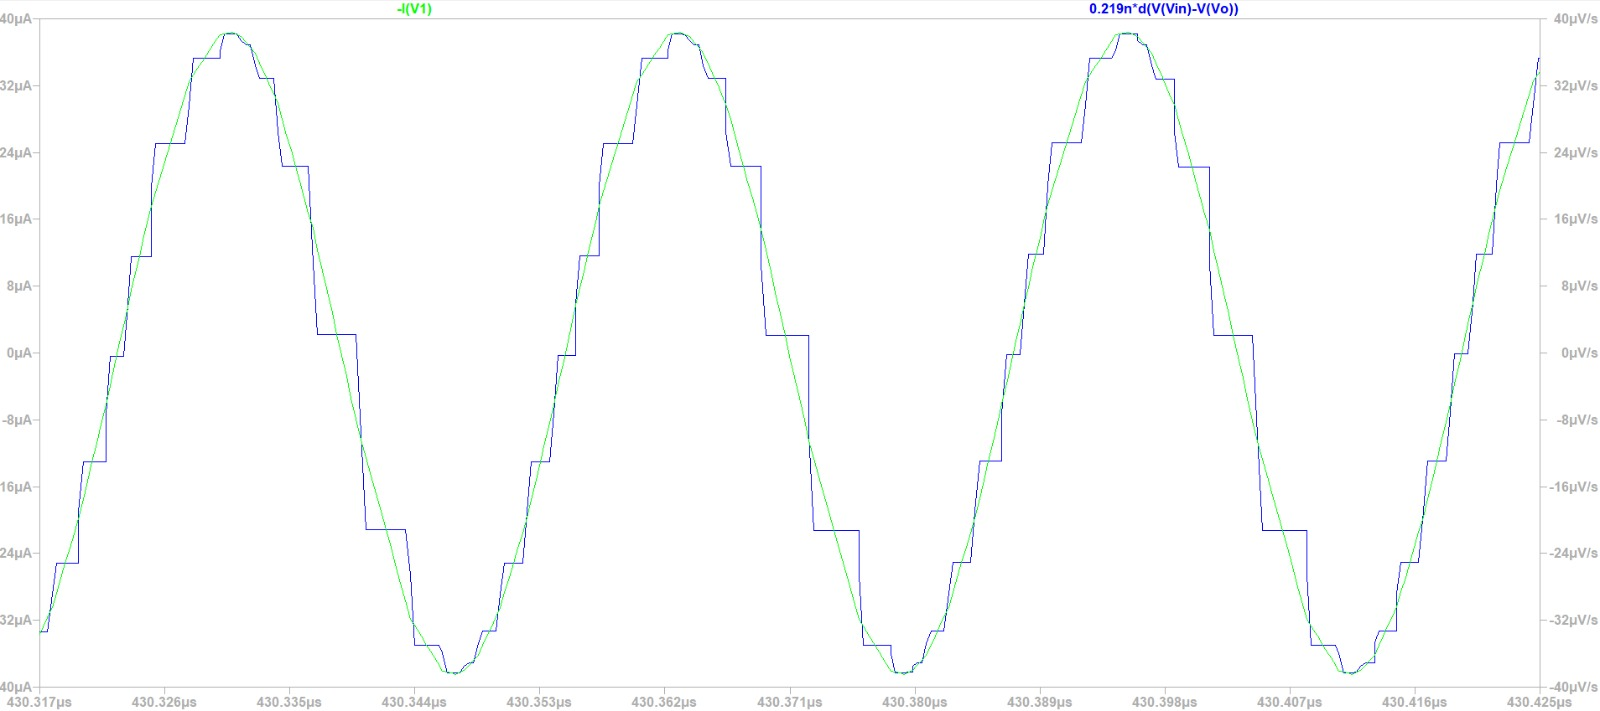
\includegraphics[scale=0.15]{figuras/fig10}
\end{figure}

Como esperado, as curvas estão em concordância.

\subsection{Varredura DC}

Essa análise é novamente realizada com o circuito divisor de corrente, para obter a corrente de $R_1$ em função da corrente da fonte, entre 0 e 0.31mA.\newpage

\begin{figure}[h]
\caption{Resultado Varredura DC}
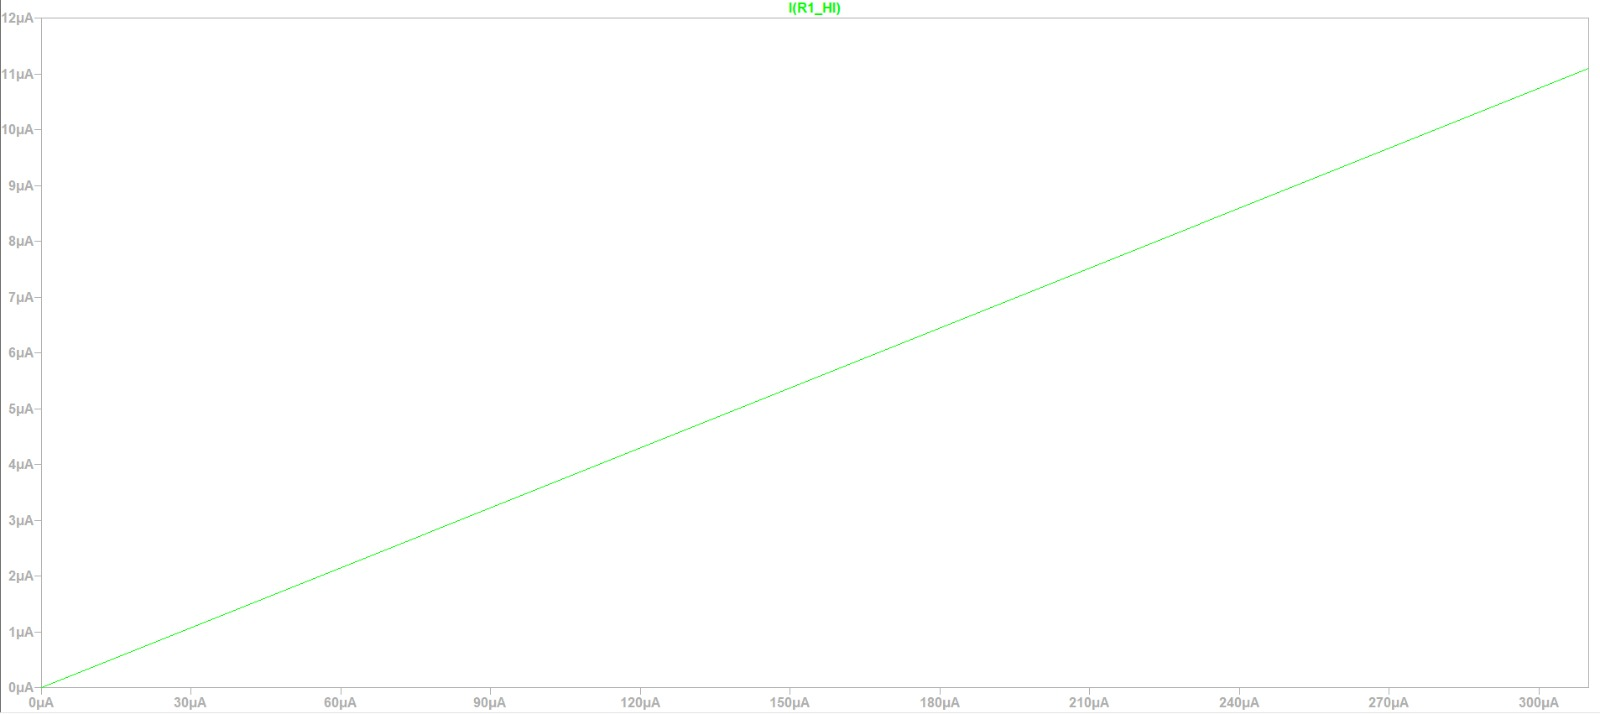
\includegraphics[scale=0.15]{figuras/fig11}
\end{figure}

\subsection{Análise da Função de Transferência}

Essa análise também é feita para o divisor de corrente, calculando a função de transferência do circuito, definida aqui como $\frac{V_{R_1}}{I_{fonte}}$. Esses valores já foram calculados na subseção \textbf{2.1} e valem: $V_{R_1} = U = 0.2883V$ e $I_{fonte} = i = 0.31mA$. Além disso, a impedância calculada na análise é simplesmente $R_{eq}$, que sabemos ser $0.93k\Omega$. Assim, temos que a função de transferência equivale a $\frac{0.2883}{0.31}\cdot10^3=930$.

Na Figura 12 está o resultado do cálculo do software. 

\begin{figure}[h]
\caption{Resultado Análise Função de Transferência}
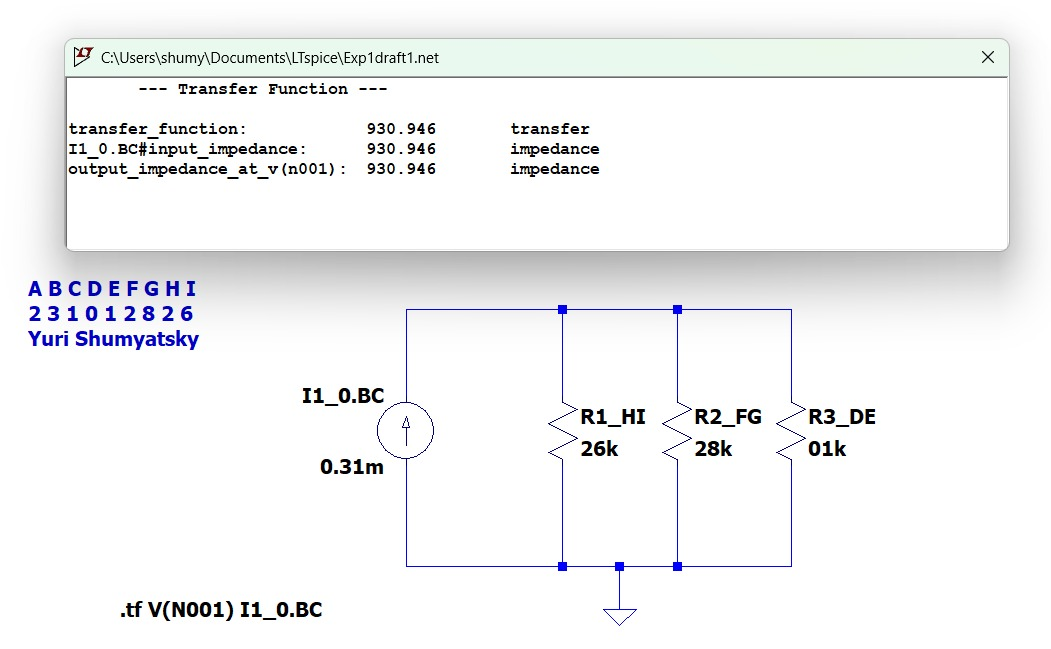
\includegraphics[scale=0.2]{figuras/fig12}
\end{figure}
%------------------------------------------------------------------------
\section{Conclusão}

Neste experimento, foi possível familiarizar-se com o uso do software LTspice para a simulação de circuitos elétricos, abrangendo análises DC, AC e transientes. A análise do divisor de corrente permitiu compreender o cálculo da resistência equivalente e a distribuição das correntes nos resistores, confirmando experimentalmente a Lei das Correntes de Kirchhoff e o Teorema de Tellegen.

Para o filtro RC passa-altas, determinou-se a capacitância necessária para atingir a frequência de corte de 28 kHz e foram obtidas as respostas em amplitude e fase através de simulação AC. A comparação entre a corrente medida no circuito e a corrente calculada pelo software mostrou excelente concordância, validando o comportamento teórico do capacitor em sinais alternados.

As análises transiente e de varredura DC reforçaram a compreensão sobre a dinâmica do circuito diante de sinais senoidais e triangulares, bem como a relação entre corrente e tensão nos elementos. A função de transferência do divisor de corrente foi confirmada numericamente, evidenciando a coerência entre teoria e simulação.


Em suma, o experimento permitiu consolidar conceitos fundamentais de circuitos elétricos e eletrônicos, a aplicação de leis básicas de corrente e tensão, e a prática de simulação computacional como ferramenta de análise. Além disso, evidenciou a importância de correlacionar cálculos teóricos com resultados simulados, reforçando a confiabilidade das simulações para o estudo de sistemas elétricos e eletrônicos.

{\small
\bibliography{egbib}
\bibliographystyle{ieee_fullname}
}

\begin{itemize}
\item Razavi, B. Fundamentos de Microeletrônica, 2\textordfeminine Edição, LTC, 2014.
\end{itemize}


\end{document}
